\documentclass[12pt,a4paper]{article}
\usepackage{physics}
\usepackage{amssymb, amsmath, graphicx}
\usepackage{subcaption}
\usepackage{svg}
\svgpath{{svg/}}
\newcommand{\activity}{Activity 17 -- Neural Networks}
\input{spp.dat}

\begin{document}

\title{\TitleFont \activity}
\author[ ]{\textbf{Kenneth V. Domingo} \\
2015--03116 \\
App Physics 186, 1\textsuperscript{st} Semester, A.Y. 2019--20}
\affil[ ]{\corremail{kvdomingo@up.edu.ph} }

\maketitle
\thispagestyle{titlestyle}

\section*{Results and Discussion}
\setcounter{section}{1}
\subsection{Function fitter}

\begin{figure}[htb]
	\centering
	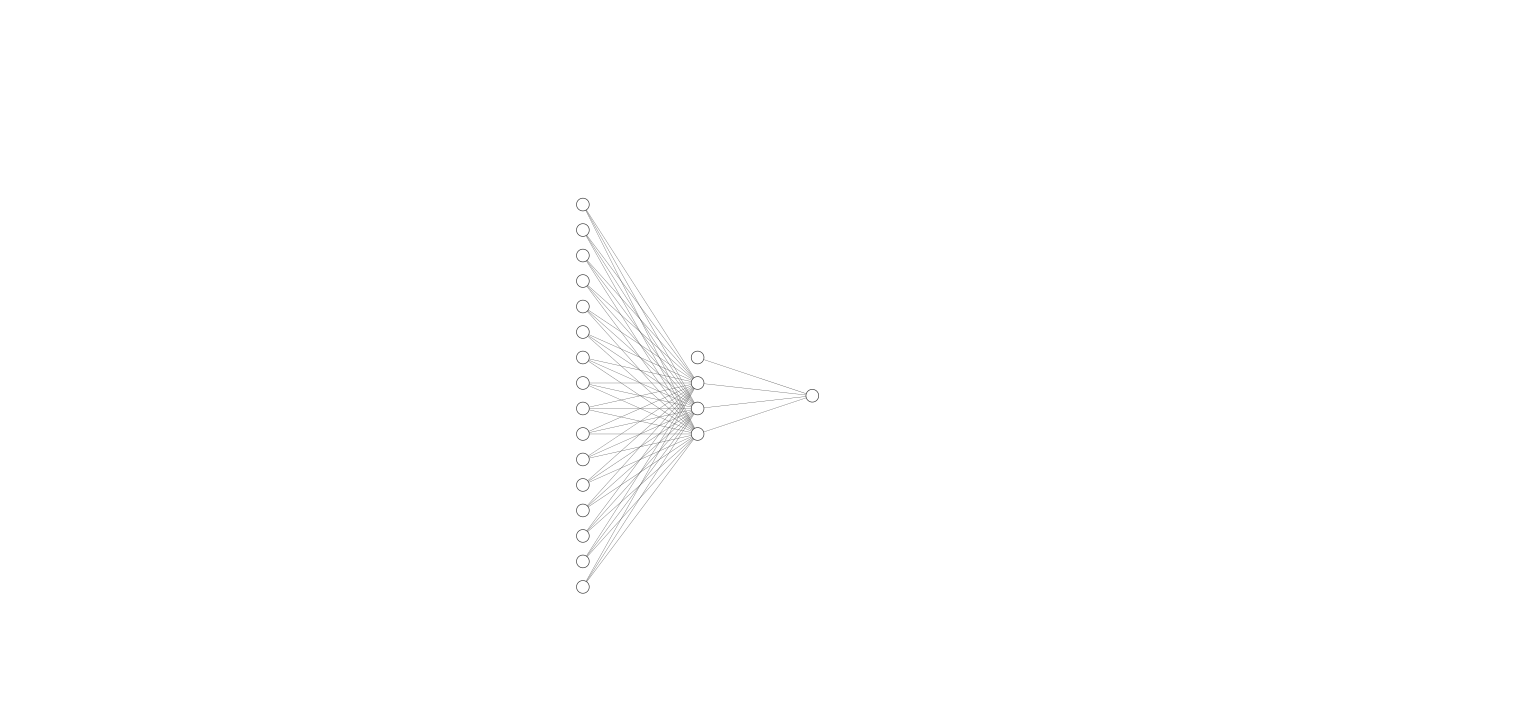
\includegraphics[width=0.75\textwidth]{func-fit.png}
	\caption{Network architecture for the function fitter.}
\end{figure}

\clearpage
\begin{table}[!htb]
	\centering
	\caption{Self-evaluation.}
	\begin{tabular}{||r|c||}
		\hline
		Technical correctness & 5 \\ \hline
		Quality of presentation & 5 \\ \hline
		Initiative & 2 \\ \hline
		\textbf{TOTAL} & \textbf{2} \\ \hline
	\end{tabular}
	\label{tab:self-eval}
\end{table}

\bibliographystyle{spp-bst}
\bibliography{biblio}

\end{document}